\documentclass{beamer}
\usepackage{lipsum}
\usepackage[utf8]{inputenc}

\usetheme{Madrid}
\usecolortheme{default}

\title[Odporúčacie systémy]{Návrh systému odporúčaní hudby}
\author[Khmelevskyi Oleksii]{Oleksii Khmelevskyi}
\institute[STU]{Slovenská technická univerzita v Bratislave\\
	Fakulta informatiky a informačných technológií
	}
\date[MIP 2024]{November 2024}


\begin{document}

\frame{\titlepage}

\begin{frame}
\frametitle{Outline}
\tableofcontents
\end{frame}

\section{Úvod}

\begin{frame}
\frametitle{Úvod}
\lipsum[1]
\end{frame}

\section{First section}

\begin{frame}
\frametitle{Diagram}
\begin{figure}
    \centering
    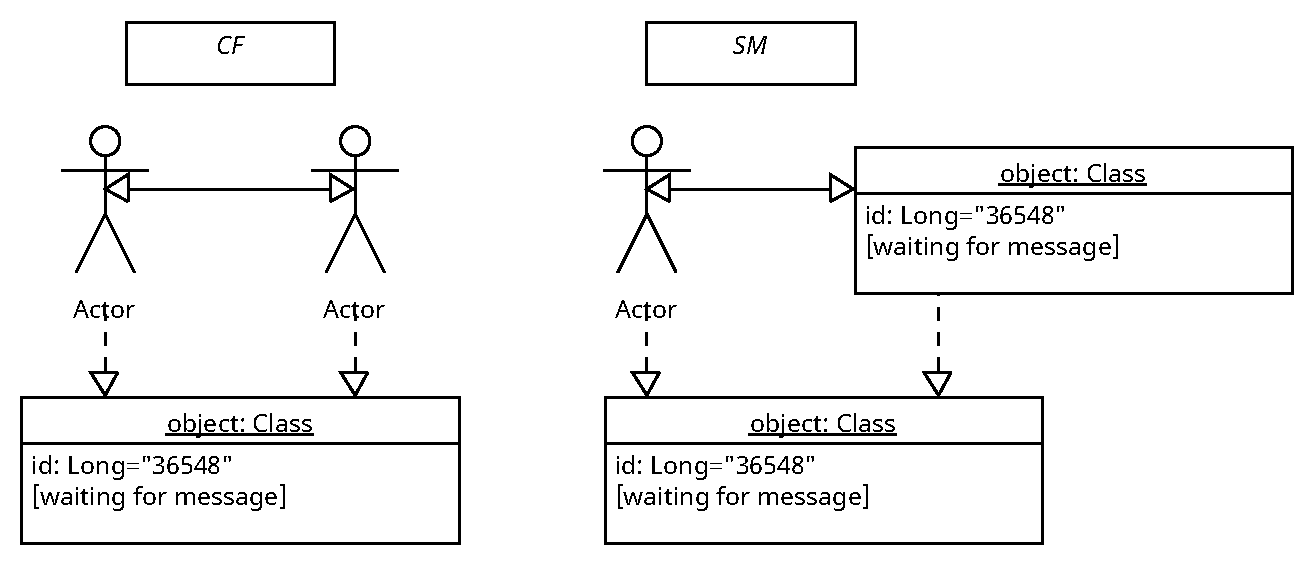
\includegraphics[width=1\linewidth]{td2.pdf}
    \caption{Collaborative filtering and similarity model}
    \label{fig:enter-label}
\end{figure}
\end{frame}
\begin{frame}
\frametitle{Zoznam}
\begin{itemize}
\item Collaborative filtering
\begin{itemize}
    \item User to user
\end{itemize}
\item Similarity model
\begin{itemize}
    \item User to content
\end{itemize}
\end{itemize}
\end{frame}

\end{document}